% $Id$

\subsection{\label{ssec:aims}Aims and Objectives}

The main project aim in this GSoC 2008 is to implement TFR(W)C over VIC, and it
can be (roughly) sub-categorized with short descriptions as belows:

\begin{enumerate} %% start enumerating

\item \textbf{TFR(W)C}

\begin{itemize}
\item \textsf{sender/receiver} -- protocol implementation 
\item \textsf{CC handler} -- generic congestion control function handler
\item \textsf{RTP for TFR(W)C} -- RTP interface with TFR(W)C
\item \textsf{RTP} -- RTP extension 
\end{itemize}

\item \textbf{Buffers}
\begin{itemize}
\item \textsf{send buffer (sbuf)} --  maintain send buffer context (e.g., frame
length, number of frames, send time to transmit a frame, and etc.)
\item \textsf{receive buffer (rbuf)} -- de-queue received frames
\end{itemize}

\item \textbf{Codecs}
\begin{itemize}
\item \textsf{video codecs} -- ability to change encoding rates based on the 
feedback information from CC mechanisms
\end{itemize}

\item \textbf{Test Modules}
\begin{itemize}
\item \textsf{packet gen} -- dummy packet generator to test TFR(W) protocol
implementation at the initial development stage
\item \textsf{traffic gen} -- traffic generator to evaluate VIC with CC
mechanisms
\end{itemize}

\end{enumerate} %% end enumerating

Roughly speaking, there are 5 components to be developed in this project: TFRC,
TFWC, Buffers, Codecs, and Test Modules. We discuss some design/development
issues in the following subsections.


\subsubsection{\label{sssec:aim:cc}TFR(W)C Implementation}

We hope that we could nicely re-use TFR(W)C implementation from
UltraGrid~\cite{UltraGrid} and ns-2 version of TFWC~\cite{SH06}, respectively.
Although the base architecture is different from what those codes, we still
think that we can refer much of their codes. However, we still do not have a
concrete idea which part can be re-used or which part cannot.

\subsubsection{\label{sssec:aim:buffers}Buffers}

The packet buffer in the current VIC implementation~\cite{AVATS} seems to be
primitive stage - i.e., it does not have fine control of the packet buffer
queue.  As we expect CC mechanisms can provide network information (and should
be able to maintain various state variables) to the upper layer (e.g., video
codecs), the extended version of the current packet buffer is necessary. But, it
is currently not decided what kind of context should be maintained in each
buffers (send buffer and receive buffer).

\subsubsection{\label{sssec:aim:codecs}Codecs} 

Firstly, we need to find appropriate video codecs that can be used with CC
mechanisms. The ideal codec can be the one which can adapts framing rate on the
fly without re-initializing it. If this is not supported in any of the current
codecs, we could modify them in a number of different ways to reflect the
feedback information from CC mechanisms. Or, we could manipulate Q-factor in
each codec on the fly based on the feedback information. Again, all of these
decision are not made yet.

\subsubsection{\label{sssec:aim:test}Test Modules}

After implementing TFR(W)C protocols, we would be faced with the point where we
need to test our implementation. There are two things involved in this
component: packet generator and traffic generator. The encoders in the current
VIC can only take YUV, JPEG, DCT, H261, and CellB Frames\footnote{See
\texttt{module.h} under VIC home directory.}. Therefore, in order to test our CC
implementation, we need to generate packets in one of those video format. Or, we
could simply use pre-recorded video sequences to transmit for the test purpose.
Next, it's necessary to generate traffic in a real network (or a dummy network)
for that purpose.

\subsection{\label{ssec:plan}Milestones}

Based on Section~\ref{ssec:aims}, we break down time scale needed to develop
each component as belows. The milestones would like more ``conceptual'' rather
than practical or tangible. The project dates listed below are only indicative
as the project will evolve based on the results being obtained while working on
it.

\paragraph{\textsf{May 26}} \underline{\textbf{GSoC Project Start}}

\paragraph{\textsf{May 31}} Finish background research and readings: VIC source
codes and UltraGrid's TFRC implementation along with RTP extension part.  The
aim here is try looking at how TFRC was implemented over a VIC-like platform
(different library and different language so it would not be possible to
directly re-use them.).

\paragraph{\textsf{Jun. 6}} Commit necessary TFRC files - e.g., TFRC
(\texttt{tfrc\_sndr.cpp, tfrc\_rcvr.cpp}, etc), RTP integration
(\texttt{rtp\_tfrc.cpp}, etc), CC handler (\texttt{cc.cpp}, etc). It would not
be necessariliy a full implementation at this stage yet.

\paragraph{\textsf{Jun. 20}} Primitive TFRC implementation. At this stage, we
should be able to send a packet using TFRC (with dummy packets).

\paragraph{\textsf{Jun. 27}} Commit necessary TFWC files. It would not be
necessariliy a full implementation at this stage yet.

\paragraph{\textsf{Juil. 4}} Primitive TFWC implementation

\paragraph{\textsf{Jul. 7}} \underline{\textbf{Mid-term Evaluation}} -- Write
interim report: what has been obtained successfully and what has not, what
should be changed for the final project goal, etc.

\paragraph{\textsf{Jul. 18}} Examine what feedback information can be used to
codecs.  (e.g., modify codecs? or use Q-factor in a specific codec?, etc)

\paragraph{\textsf{Jul. 25}} Finalizing TFR(W)C interactioin with codecs.

\paragraph{\textsf{Aug. 1}} Test and Evaluation for the whole systems.

\paragraph{\textsf{Aug. 8}} Final evaluation and discussion

\paragraph{\textsf{Aug. 15}} Come up with final version of source codes and a
report.

\paragraph{\textsf{Aug. 18}} \underline{\textbf{Project Submission}}-- Submit
the results to Google and wrap-up.

\newpage

\subsection{\label{ssec:proposed-arch}Proposed Architecture}

We have drawn our proposed VIC architecture (sender only) that has congestion
control modules as in Figure~\ref{fig:proposed-arch}. This figure represents a
high-level overview of VIC so that we could see the major components of the
system, and how they are interacting with each other. 

\vspace{1cm}

\begin{figure}[!h]
\begin{center}
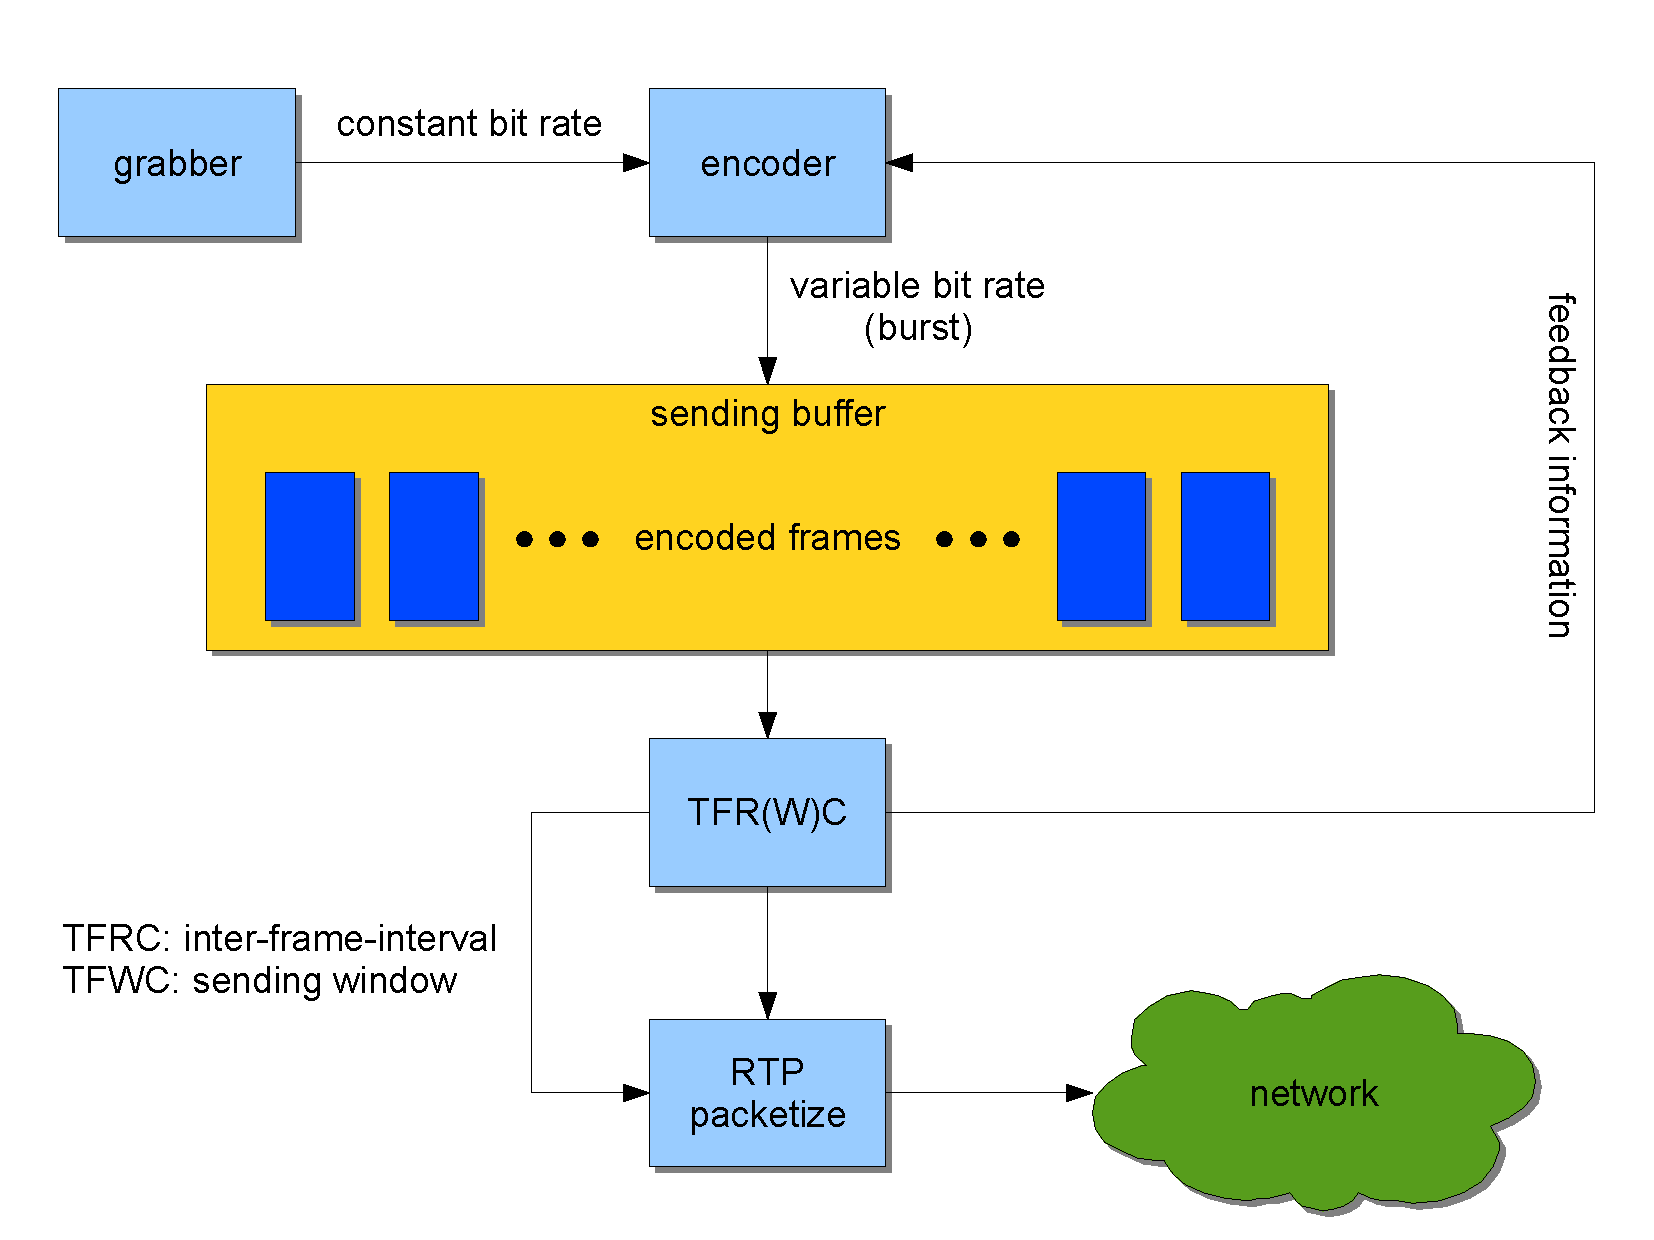
\includegraphics[scale=.5]{./img/proposed-vic-arch}
\label{fig:proposed-arch}
\caption{Proposed VIC architecture with CC mechanisms}
\end{center}
\end{figure}

Unlike to the sender, we envisage the architecture of the receiver is relatively
simple. For example, upon a packet reception, it will be inserted to a receive
buffer, subsequently decoded (and some color conversion if necessary), and
finally displayed in a output device. Depending upon a codec, the rendered
frames may not be discareded immediately, but will be kept for some times before
they get purged.

\newpage
